% !TEX root = ../main.tex

\chapter{Technical development} % (fold)
\label{chp:execution}

\section{Terminology}
\label{sec:terminology}

The Algolia API is pushing by uploading schemaless JSON objects to an index

\section{Organizing state} % (fold)
\label{sec:organizing_state}

\subsection{Widgets and connectors}
\label{sub:widgets_and_connectors}

The big difference between using Algolia with the Helper compared to InstantSearch is the notion of widgets. In the current implementations there are ten core widgets. Each of these widgets is split up in its logic (a connector) and its display logic (a component). Together these widgets are:

\begin{itemize}
  \item SearchBox
  \item Hits
  \item RefinementList
  \item Range
  \item Pagination
  \item ClearAll
  \item CurrentRefinements
  \item Sort By
  \item Highlight
  \item Snippet
\end{itemize}

There are two kinds of widgets, interactive widgets and display-only widgets. Display-only widgets read the current results and applied refinements from the Algolia response. The display-only widgets are Hits, which is a representation of all the results. The other two are Highlight and Snippet, which take an attributen, and display the snipped and highlighted result from the Algolia response.

The other widgets are interactive widgets. They also take their display value from the response, to show which facets are enabled, or which refinement is already made. All of them also expose a {\tt refine()} function. This function will be called whenever is applicable in that case, and uses Helper methods like {\tt helper.state.toggleRefinement} to actually apply their change on the search state.

%%
talk about the difference between storing parameters and storing widget state

\subsection{Structuring a state container}
\label{sub:structuring_a_state_container}

In the InstantSearch Core implementation the choice has been made to structure state in three divisions. One for the result that comes from each API call, one for raw parameters like {\tt DISTINCT} and another division for the actual refinements.

Since InstantSearch Core is a JavaScript library, there isn't much choice for a container. A {\tt Map}\cite{mdn-map} could be used as the actual value for the {\tt result} key, but since it's not widely supported and has a significantly less elegant API, and they generally consume more memory in smaller objects. Since in the general case, Algolia results contain about 20 hits, and a finite amount of filters, using {\tt Object} is perfectly reasonable.

\begin{lstlisting}[caption={The state container of InstantSearch Core},label={lst:is-core-state-1}]
const state = {
  refinements,
  rawParameters,
  result,
};
\end{lstlisting}

Here, the most interesting container is the {\tt refinements} container. It's structured as another {\tt Object} with a key for every attribute name which is being refined, and is inspired by the structure of the state {\tt Object} in React InstantSearch\cite{react-instantsearch-search-state}.

Every attribute is another {\tt Object}, with a {\tt type} key, and a {\tt value} key. For each of the possible refinements, a value that is relevant is chosen. 

A menu for example is a refinement that takes a attribute that has been set up for faceting\cite{algolia-set-up-faceting} and has a single value. For that reason a menu takes in a string as a value. A list is a refinement that is exactly the same, but takes a list of strings to be able to set up multiple refined values for that attribute.

Having a structure like this implies that it is trivial to see if any refinements have been set, including the query. This is useful for when an interface is constructed that only shows a search bar until the first character is typed. After that a more elaborate interface shows up to fill the screen with other filters.

If every refinement would be set, the refinements key of the search state would be:

\begin{lstlisting}[caption={Refinements in InstantSearch Core},label={lst:is-core-state-2}]
const refinements = {
  color: {
    type: 'menu',
    value: 'blue',
  },
  products: {
    type: 'hierarchicalMenu',
    value: 'Laptops > Surface',
  },
  brand: {
    type: 'list',
    value: ['apple', 'samsung'],
  },
  price: {
    type: 'range',
    value: {
      min: 20,
      max: 3000
    },
  },
  freeShipping: {
    type: 'toggle',
    value: false,
  },
  query: {
    type: 'query',
    value: 'pizza',
  },
  page: {
    type: 'page',
    value: 1,
  },
};
\end{lstlisting}

To be able to handle a lot of cases that can't be foreseen by the refinements, or to handle settings that aren't visible to the user, a {\tt rawParameters} key is available in the search state. There are some 

\begin{lstlisting}[caption={Passing raw Algolia parameters to InstantSearch Core},label={lst:is-core-state-3}]
const rawParameters = {
  distinct: true,
  page: 3,
};
\end{lstlisting}

Finally, very important are the results. These results are not exactly the same as how they come in from the Algolia API. The differentiator is that there is a slight reordering to match the structure of the {\tt refinements} block.

This solves an interesting problem with InstantSearch.js. Whenever something needs to be done which isn't provided by the library, a so-called custom widget needs to be written. To be able to %%

\begin{lstlisting}[caption={Results container in the InstantSearch Core state},label={lst:is-core-state-4}]
const result = {
  color: {
    type: 'menu',
    value: [
      {
        label: 'red',
        count: 10,
      },
      {
        label: 'blue',
        count: 100,
      },
    ],
  },
  (*@{\vdots}@*)
  hits: [
    {
      objectID: '0x1f355',
      color: 'blue',
     (*@{\vdots}@*)
    },
    (*@{\vdots}@*)
  ],
  meta: { 
    processingTimeMS: 5,
    (*@{\vdots}@*)
  },
};
\end{lstlisting}

Because of this structure, a connector can be made for every refinement. It takes

connectors are easier when you can just have one listener / changer per connector type. Don't care about the global state basically.

% section organizing_state (end)

\section{Handling state changes} % (fold)
\label{sec:handling_state_changes}

%%
Research:

\begin{itemize}
  \item observables vs flux
  \item Other languages (Elm model)\cite{csstricks-elm}
\end{itemize}

% section handling_state_changes (end)

\section{Getting responses from the API} % (fold)
\label{sec:getting_responses_from_the_api}

another function listens to changes in state

it transforms params into a JS client request

it replaces the {\tt response} in the state with an action

% section getting_responses_from_the_api (end)

\section{Rendering refinements} % (fold)
\label{sec:rendering_refinements}

Stuff to think about: dynamic facets as core part of this API or not?

% section rendering_refinements (end)

\section{Saved state} % (fold)
\label{sec:saved_state}

The API also allows for an initialisation with a certain state passed in. This means that it's possible to save a state object in a location, and then later restart the search from that data. 

This is useful for three major use cases. The first is URL synchronisation. For URL synchronisation the structure would be to first listen on every state change with {\tt .subscribe()}, and then asynchronously transform that to query parameters to set. If a user comes to a page with query parameters, a function to take in the query string and put out a state object would then be called. After that point a new InstantSearch Core instance can be built with the {\tt preloadedState} parameter set in the constructor.

INSERT: image to show how URL-sync should be implemented

Similarly it is also possible to do that process with a different medium than query parameters, for example {\tt localStorage}. For that reason this process is left over to the user, possibly with other small packages dealing with browser inconsistencies on top of it. 

This pattern is also useful for when Server Side Rendering (SSR) is implemented. When ...

\begin{enumerate}
  \item execute the IS function once
  \item render the output as html
  \item also output the state object in a global object
  \item send that html to the client
  \item start the IS instance frontend with preloadedState: {\tt window.PRELOADED\_STATE}
\end{enumerate}

INSERT: image to show how SSR should be implemented

% section saved_state (end)

\section{Overview} % (fold)
\label{sec:overview}

\begin{figure}[H]
\label{figure:core-architecture}
  \centering
  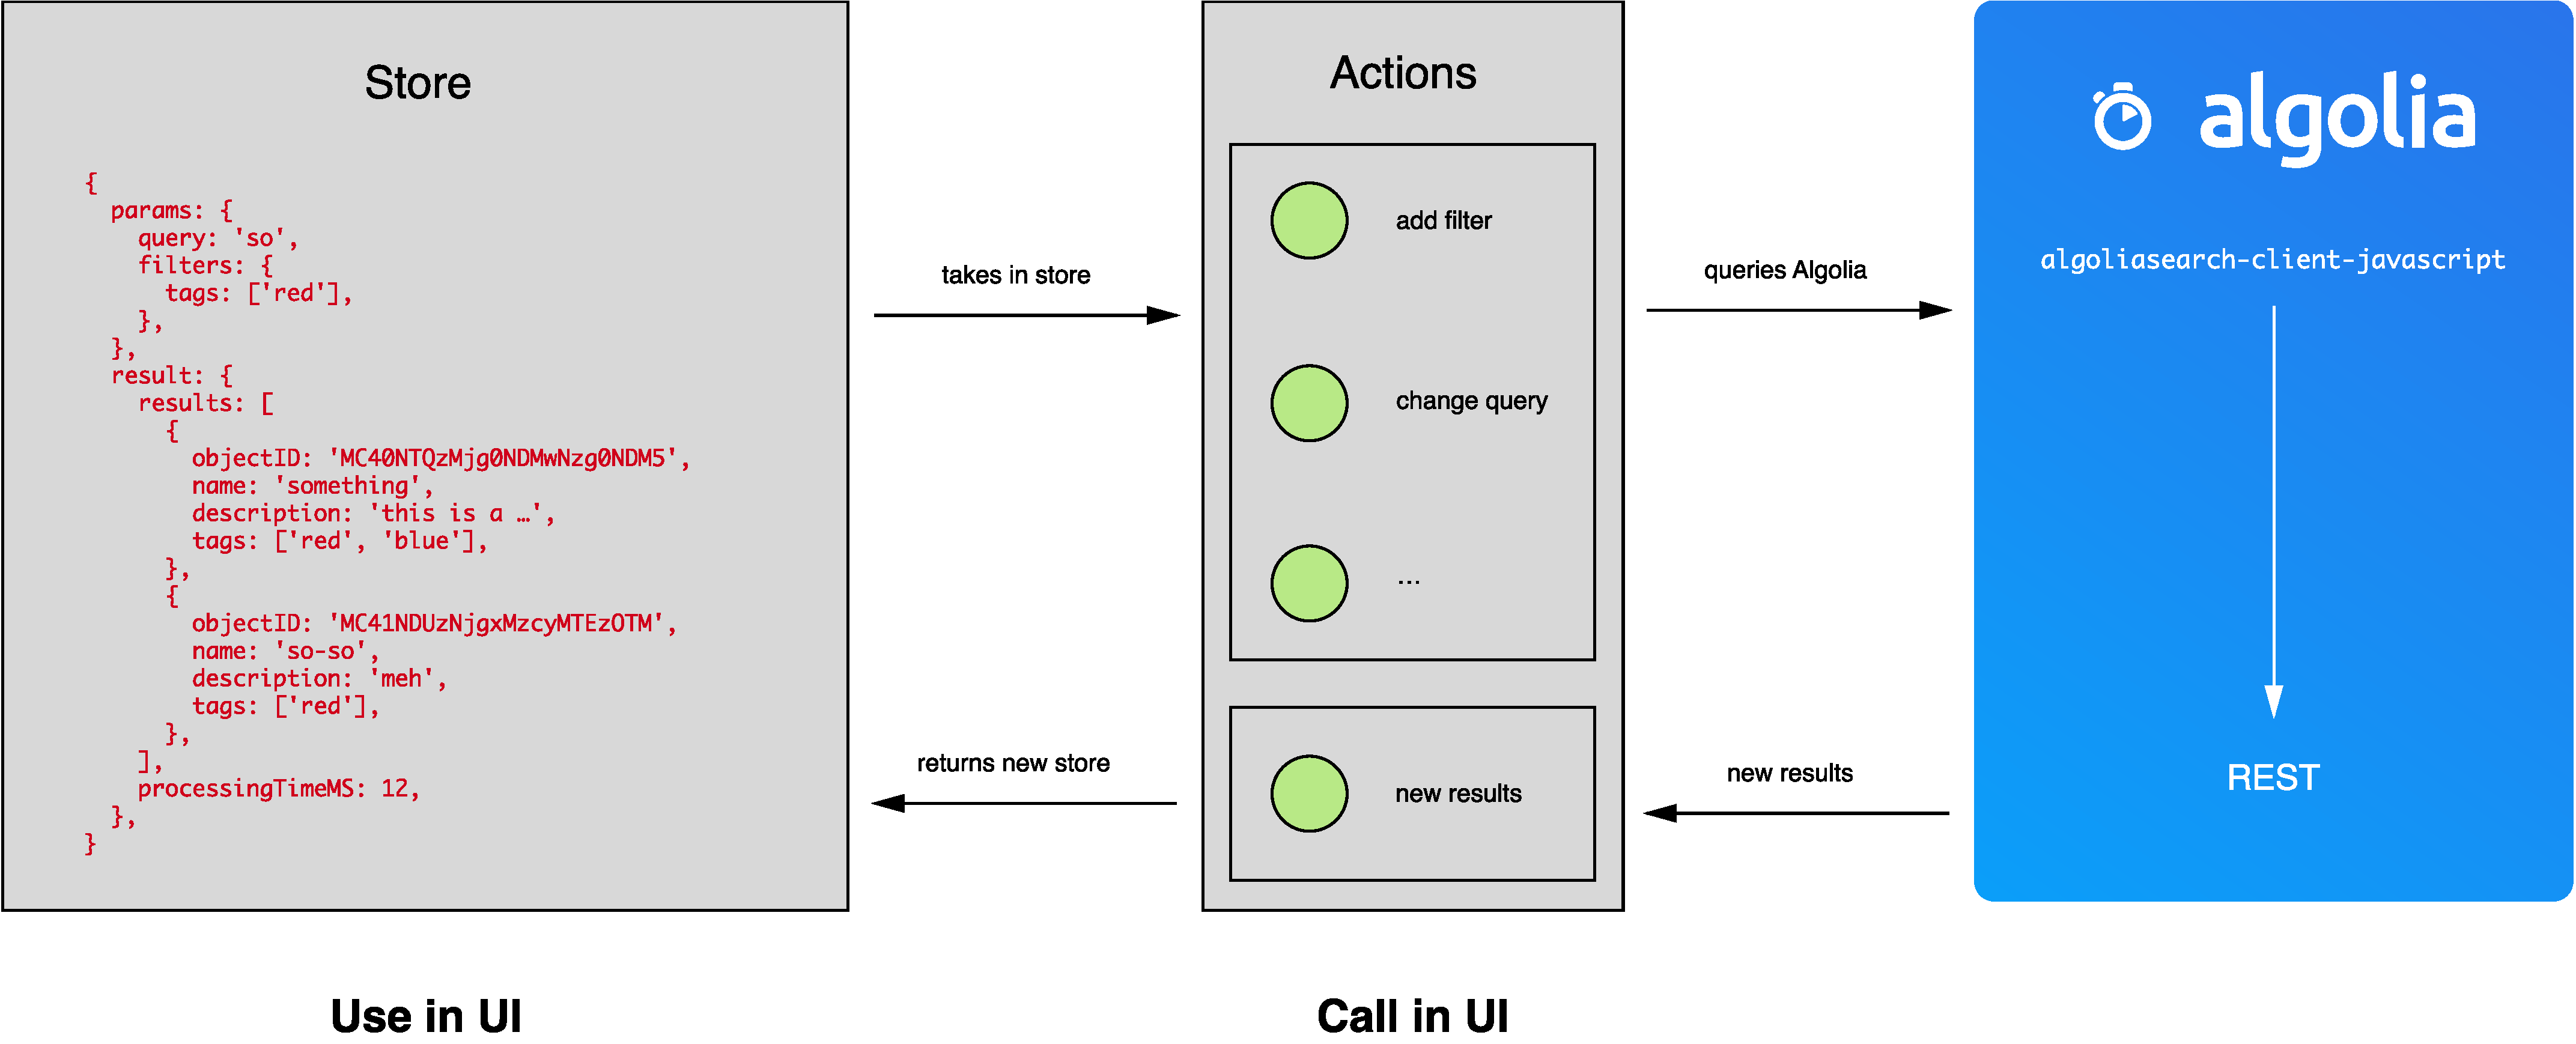
\includegraphics[width=\textwidth]{../assets/architecture.pdf}
  \caption{Architecture overview\cite{blog-architecture}}
\end{figure}

TODO: update this image with more recent architecture

% section overview (end)

\section{Usage in libraries} % (fold)
\label{sec:usage_in_libraries}

PoC in instantsearch.js and ReactInstantsearch for the RefinementList %%

% section usage_in_libraries (end)

\section{Complete implementation} % (fold)
\label{sec:complete_implementation}

Obviously this isn't final and too detailed.

\begin{lstlisting}[caption={Using instantsearch-core},label={lst:is-core-usage}]
// stores.js
import algoliasearch from 'algoliasearch';
import { createStore } from 'instantsearch-core';

const appId = 'OFCNCOG2CU';
const apiKey = 'f54e21fa3a2a0160595bb058179bfb1e';
const indexName = 'products_asc';

const client = algoliasearch(appId, apiKey);
const productsStore = createStore(client, indexName);

export productsStore;

// widget.js
import { setQuery } from 'instantsearch-core/actions/query';
import { productsStore } from './stores';

function onInput(event) {
  event.preventDefault();

  productsStore.refine(setQuery(event.target.value));
}
\end{lstlisting}

% section complete_implementation (end)

